%% bare_conf.tex
%% V1.3
%% 2007/01/11
%% by Michael Shell
%% See:
%% http://www.michaelshell.org/
%% for current contact information.
%%
%% This is a skeleton file demonstrating the use of IEEEtran.cls
%% (requires IEEEtran.cls version 1.7 or later) with an IEEE conference paper.
%%
%% Support sites:
%% http://www.michaelshell.org/tex/ieeetran/
%% http://www.ctan.org/tex-archive/macros/latex/contrib/IEEEtran/
%% and
%% http://www.ieee.org/

%%*************************************************************************
%% Legal Notice:
%% This code is offered as-is without any warranty either expressed or
%% implied; without even the implied warranty of MERCHANTABILITY or
%% FITNESS FOR A PARTICULAR PURPOSE! 
%% User assumes all risk.
%% In no event shall IEEE or any contributor to this code be liable for
%% any damages or losses, including, but not limited to, incidental,
%% consequential, or any other damages, resulting from the use or misuse
%% of any information contained here.
%%
%% All comments are the opinions of their respective authors and are not
%% necessarily endorsed by the IEEE.
%%
%% This work is distributed under the LaTeX Project Public License (LPPL)
%% ( http://www.latex-project.org/ ) version 1.3, and may be freely used,
%% distributed and modified. A copy of the LPPL, version 1.3, is included
%% in the base LaTeX documentation of all distributions of LaTeX released
%% 2003/12/01 or later.
%% Retain all contribution notices and credits.
%% ** Modified files should be clearly indicated as such, including  **
%% ** renaming them and changing author support contact information. **
%%
%% File list of work: IEEEtran.cls, IEEEtran_HOWTO.pdf, bare_adv.tex,
%%                    bare_conf.tex, bare_jrnl.tex, bare_jrnl_compsoc.tex
%%*************************************************************************

% *** Authors should verify (and, if needed, correct) their LaTeX system  ***
% *** with the testflow diagnostic prior to trusting their LaTeX platform ***
% *** with production work. IEEE's font choices can trigger bugs that do  ***
% *** not appear when using other class files.                            ***
% The testflow support page is at:
% http://www.michaelshell.org/tex/testflow/



% Note that the a4paper option is mainly intended so that authors in
% countries using A4 can easily print to A4 and see how their papers will
% look in print - the typesetting of the document will not typically be
% affected with changes in paper size (but the bottom and side margins will).
% Use the testflow package mentioned above to verify correct handling of
% both paper sizes by the user's LaTeX system.
%
% Also note that the "draftcls" or "draftclsnofoot", not "draft", option
% should be used if it is desired that the figures are to be displayed in
% draft mode.
%
\documentclass[conference]{IEEEtran}
% Add the compsoc option for Computer Society conferences.
%
% If IEEEtran.cls has not been installed into the LaTeX system files,
% manually specify the path to it like:
% \documentclass[conference]{../sty/IEEEtran}





% Some very useful LaTeX packages include:
% (uncomment the ones you want to load)


% *** MISC UTILITY PACKAGES ***
%
%\usepackage{ifpdf}
% Heiko Oberdiek's ifpdf.sty is very useful if you need conditional
% compilation based on whether the output is pdf or dvi.
% usage:
% \ifpdf
%   % pdf code
% \else
%   % dvi code
% \fi
% The latest version of ifpdf.sty can be obtained from:
% http://www.ctan.org/tex-archive/macros/latex/contrib/oberdiek/
% Also, note that IEEEtran.cls V1.7 and later provides a builtin
% \ifCLASSINFOpdf conditional that works the same way.
% When switching from latex to pdflatex and vice-versa, the compiler may
% have to be run twice to clear warning/error messages.





%*** Citation Package ***
\usepackage[numbers]{natbib}
\usepackage{url}


% *** GRAPHICS RELATED PACKAGES ***
%
\ifCLASSINFOpdf
  \usepackage[pdftex]{graphicx}
  % declare the path(s) where your graphic files are
  \graphicspath{{../pdf/}{../jpeg/}{figures}}
  % and their extensions so you won't have to specify these with
  % every instance of \includegraphics
  \DeclareGraphicsExtensions{.pdf,.jpeg,.png}
\else
  % or other class option (dvipsone, dvipdf, if not using dvips). graphicx
  % will default to the driver specified in the system graphics.cfg if no
  % driver is specified.
  % \usepackage[dvips]{graphicx}
  % declare the path(s) where your graphic files are
  % \graphicspath{{../eps/}}
  % and their extensions so you won't have to specify these with
  % every instance of \includegraphics
  % \DeclareGraphicsExtensions{.eps}
\fi
% graphicx was written by David Carlisle and Sebastian Rahtz. It is
% required if you want graphics, photos, etc. graphicx.sty is already
% installed on most LaTeX systems. The latest version and documentation can
% be obtained at: 
% http://www.ctan.org/tex-archive/macros/latex/required/graphics/
% Another good source of documentation is "Using Imported Graphics in
% LaTeX2e" by Keith Reckdahl which can be found as epslatex.ps or
% epslatex.pdf at: http://www.ctan.org/tex-archive/info/
%
% latex, and pdflatex in dvi mode, support graphics in encapsulated
% postscript (.eps) format. pdflatex in pdf mode supports graphics
% in .pdf, .jpeg, .png and .mps (metapost) formats. Users should ensure
% that all non-photo figures use a vector format (.eps, .pdf, .mps) and
% not a bitmapped formats (.jpeg, .png). IEEE frowns on bitmapped formats
% which can result in "jaggedy"/blurry rendering of lines and letters as
% well as large increases in file sizes.
%
% You can find documentation about the pdfTeX application at:
% http://www.tug.org/applications/pdftex





% *** MATH PACKAGES ***
%
%\usepackage[cmex10]{amsmath}
% A popular package from the American Mathematical Society that provides
% many useful and powerful commands for dealing with mathematics. If using
% it, be sure to load this package with the cmex10 option to ensure that
% only type 1 fonts will utilized at all point sizes. Without this option,
% it is possible that some math symbols, particularly those within
% footnotes, will be rendered in bitmap form which will result in a
% document that can not be IEEE Xplore compliant!
%
% Also, note that the amsmath package sets \interdisplaylinepenalty to 10000
% thus preventing page breaks from occurring within multiline equations. Use:
%\interdisplaylinepenalty=2500
% after loading amsmath to restore such page breaks as IEEEtran.cls normally
% does. amsmath.sty is already installed on most LaTeX systems. The latest
% version and documentation can be obtained at:
% http://www.ctan.org/tex-archive/macros/latex/required/amslatex/math/





% *** SPECIALIZED LIST PACKAGES ***
%
%\usepackage{algorithmic}
% algorithmic.sty was written by Peter Williams and Rogerio Brito.
% This package provides an algorithmic environment fo describing algorithms.
% You can use the algorithmic environment in-text or within a figure
% environment to provide for a floating algorithm. Do NOT use the algorithm
% floating environment provided by algorithm.sty (by the same authors) or
% algorithm2e.sty (by Christophe Fiorio) as IEEE does not use dedicated
% algorithm float types and packages that provide these will not provide
% correct IEEE style captions. The latest version and documentation of
% algorithmic.sty can be obtained at:
% http://www.ctan.org/tex-archive/macros/latex/contrib/algorithms/
% There is also a support site at:
% http://algorithms.berlios.de/index.html
% Also of interest may be the (relatively newer and more customizable)
% algorithmicx.sty package by Szasz Janos:
% http://www.ctan.org/tex-archive/macros/latex/contrib/algorithmicx/




% *** ALIGNMENT PACKAGES ***
%
%\usepackage{array}
% Frank Mittelbach's and David Carlisle's array.sty patches and improves
% the standard LaTeX2e array and tabular environments to provide better
% appearance and additional user controls. As the default LaTeX2e 
% generation code is lacking to the point of almost being broken with
% respect to the quality of the end results, all users are strongly
% advised to use an enhanced (at the very least that provided by array.sty)
% set of table tools. array.sty is already installed on most systems. The
% latest version and documentation can be obtained at:
% http://www.ctan.org/tex-archive/macros/latex/required/tools/


%\usepackage{mdwmath}
%\usepackage{mdwtab}
% Also highly recommended is Mark Wooding's extremely powerful MDW tools,
% especially mdwmath.sty and mdwtab.sty which are used to format equations
% and tables, respectively. The MDWtools set is already installed on most
% LaTeX systems. The lastest version and documentation is available at:
% http://www.ctan.org/tex-archive/macros/latex/contrib/mdwtools/


% IEEEtran contains the IEEEeqnarray family of commands that can be used to
% generate multiline equations as well as matrices, tables, etc., of high
% quality.


%\usepackage{eqparbox}
% Also of notable interest is Scott Pakin's eqparbox package for creating
% (automatically sized) equal width boxes - aka "natural width parboxes".
% Available at:
% http://www.ctan.org/tex-archive/macros/latex/contrib/eqparbox/





% *** SUBFIGURE PACKAGES ***
%\usepackage[tight,footnotesize]{subfigure}
% subfigure.sty was written by Steven Douglas Cochran. This package makes it
% easy to put subfigures in your figures. e.g., "Figure 1a and 1b". For IEEE
% work, it is a good idea to load it with the tight package option to reduce
% the amount of white space around the subfigures. subfigure.sty is already
% installed on most LaTeX systems. The latest version and documentation can
% be obtained at:
% http://www.ctan.org/tex-archive/obsolete/macros/latex/contrib/subfigure/
% subfigure.sty has been superceeded by subfig.sty.



%\usepackage[caption=false]{caption}
%\usepackage[font=footnotesize]{subfig}
% subfig.sty, also written by Steven Douglas Cochran, is the modern
% replacement for subfigure.sty. However, subfig.sty requires and
% automatically loads Axel Sommerfeldt's caption.sty which will override
% IEEEtran.cls handling of captions and this will result in nonIEEE style
% figure/table captions. To prevent this problem, be sure and preload
% caption.sty with its "caption=false" package option. This is will preserve
% IEEEtran.cls handing of captions. Version 1.3 (2005/06/28) and later 
% (recommended due to many improvements over 1.2) of subfig.sty supports
% the caption=false option directly:
%\usepackage[caption=false,font=footnotesize]{subfig}
%
% The latest version and documentation can be obtained at:
% http://www.ctan.org/tex-archive/macros/latex/contrib/subfig/
% The latest version and documentation of caption.sty can be obtained at:
% http://www.ctan.org/tex-archive/macros/latex/contrib/caption/




% *** FLOAT PACKAGES ***
%
%\usepackage{fixltx2e}
% fixltx2e, the successor to the earlier fix2col.sty, was written by
% Frank Mittelbach and David Carlisle. This package corrects a few problems
% in the LaTeX2e kernel, the most notable of which is that in current
% LaTeX2e releases, the ordering of single and double column floats is not
% guaranteed to be preserved. Thus, an unpatched LaTeX2e can allow a
% single column figure to be placed prior to an earlier double column
% figure. The latest version and documentation can be found at:
% http://www.ctan.org/tex-archive/macros/latex/base/



%\usepackage{stfloats}
% stfloats.sty was written by Sigitas Tolusis. This package gives LaTeX2e
% the ability to do double column floats at the bottom of the page as well
% as the top. (e.g., "\begin{figure*}[!b]" is not normally possible in
% LaTeX2e). It also provides a command:
%\fnbelowfloat
% to enable the placement of footnotes below bottom floats (the standard
% LaTeX2e kernel puts them above bottom floats). This is an invasive package
% which rewrites many portions of the LaTeX2e float routines. It may not work
% with other packages that modify the LaTeX2e float routines. The latest
% version and documentation can be obtained at:
% http://www.ctan.org/tex-archive/macros/latex/contrib/sttools/
% Documentation is contained in the stfloats.sty comments as well as in the
% presfull.pdf file. Do not use the stfloats baselinefloat ability as IEEE
% does not allow \baselineskip to stretch. Authors submitting work to the
% IEEE should note that IEEE rarely uses double column equations and
% that authors should try to avoid such use. Do not be tempted to use the
% cuted.sty or midfloat.sty packages (also by Sigitas Tolusis) as IEEE does
% not format its papers in such ways.

%multirow tables. example: http://maksim.sorokin.dk/it/2010/05/22/multirow-and-multicolumn-spanning-in-latex/
\usepackage{multirow}



% *** PDF, URL AND HYPERLINK PACKAGES ***
%
%\usepackage{url}
% url.sty was written by Donald Arseneau. It provides better support for
% handling and breaking URLs. url.sty is already installed on most LaTeX
% systems. The latest version can be obtained at:
% http://www.ctan.org/tex-archive/macros/latex/contrib/misc/
% Read the url.sty source comments for usage information. Basically,
% \url{my_url_here}.





% *** Do not adjust lengths that control margins, column widths, etc. ***
% *** Do not use packages that alter fonts (such as pslatex).         ***
% There should be no need to do such things with IEEEtran.cls V1.6 and later.
% (Unless specifically asked to do so by the journal or conference you plan
% to submit to, of course. )


% correct bad hyphenation here
\hyphenation{vis-ual lang-u-ages}


\begin{document}
%
% paper title
% can use linebreaks \\ within to get better formatting as desired
\title{Measuring the Programmatic Sophistication of App Inventor Projects Grouped by Functionality}


% author names and affiliations
% use a multiple column layout for up to three different
% affiliations
\author{\IEEEauthorblockN{Benjamin Xie, Isra Shabir, and Hal Abelson}
\IEEEauthorblockA{Department of Electrical Engineering and Computer Science\\
Massachusetts Institute of Technology\\
Cambridge, Massachusetts, USA\\
Email: \{bxie, ishabir, hal\}@mit.edu}}
%\and
%\IEEEauthorblockN{Isra Shabir}
%\IEEEauthorblockA{Department of Electrical Engineering\\and Computer Science\\
%Massachusetts Institute of Technology\\
%Cambridge, Massachusetts 02139\\
%Email: ishabir@mit.edu}
%\and
%\IEEEauthorblockN{James Kirk\\ and Montgomery Scott}
%\IEEEauthorblockA{Starfleet Academy\\
%San Francisco, California 96678-2391\\
%Telephone: (800) 555--1212\\
%Fax: (888) 555--1212}}

% conference papers do not typically use \thanks and this command
% is locked out in conference mode. If really needed, such as for
% the acknowledgment of grants, issue a \IEEEoverridecommandlockouts
% after \documentclass

% for over three affiliations, or if they all won't fit within the width
% of the page, use this alternative format:
% 
%\author{\IEEEauthorblockN{Michael Shell\IEEEauthorrefmark{1},
%Homer Simpson\IEEEauthorrefmark{2},
%James Kirk\IEEEauthorrefmark{3}, 
%Montgomery Scott\IEEEauthorrefmark{3} and
%Eldon Tyrell\IEEEauthorrefmark{4}}
%\IEEEauthorblockA{\IEEEauthorrefmark{1}School of Electrical and Computer Engineering\\
%Georgia Institute of Technology,
%Atlanta, Georgia 30332--0250\\ Email: see http://www.michaelshell.org/contact.html}
%\IEEEauthorblockA{\IEEEauthorrefmark{2}Twentieth Century Fox, Springfield, USA\\
%Email: homer@thesimpsons.com}
%\IEEEauthorblockA{\IEEEauthorrefmark{3}Starfleet Academy, San Francisco, California 96678-2391\\
%Telephone: (800) 555--1212, Fax: (888) 555--1212}
%\IEEEauthorblockA{\IEEEauthorrefmark{4}Tyrell Inc., 123 Replicant Street, Los Angeles, California 90210--4321}}




% use for special paper notices
%\IEEEspecialpapernotice{(Invited Paper)}




% make the title area
\maketitle


\begin{abstract}
%\boldmath
MIT App Inventor is a web service that enables users with little to no previous programming experience to create mobile applications using a visual blocks language. We analyze a sample of 5,228 random projects from the corpus of 8.3 million and group projects by functionality. We then use the number of unique blocks in projects and measure the programmatic sophistication of apps to better understand the learnability and realized capability of using App Inventor to implement specific functionalities. We introduce the notion of a learnability score and our results indicate that introductory tutorials heavily influence the learnability of particular functionalities with App Inventor. Our findings suggest that the sequential nature of App Inventor’s learning resources results in users realizing only a portion of App Inventor’s capabilities and propose improvements to these resources.
\end{abstract}
% IEEEtran.cls defaults to using nonbold math in the Abstract.
% This preserves the distinction between vectors and scalars. However,
% if the conference you are submitting to favors bold math in the abstract,
% then you can use LaTeX's standard command \boldmath at the very start
% of the abstract to achieve this. Many IEEE journals/conferences frown on
% math in the abstract anyway.

% no keywords




% For peer review papers, you can put extra information on the cover
% page as needed:
% \ifCLASSOPTIONpeerreview
% \begin{center} \bfseries EDICS Category: 3-BBND \end{center}
% \fi
%
% For peerreview papers, this IEEEtran command inserts a page break and
% creates the second title. It will be ignored for other modes.
\IEEEpeerreviewmaketitle



\section{Introduction}

% no \IEEEPARstart


% You must have at least 2 lines in the paragraph with the drop letter
% (should never be an issue)


%\hfill mds
 
%\hfill April 3, 2015

%\subsection{MIT App Inventor}
MIT App Inventor is an environment that leverages a blocks-based visual programming language to enable people to create mobile apps for Android devices \cite{ai_home}. An App Inventor project consists of a set of components and a set of program blocks that enable the functionality of these components. Components include items visible on the phone screen (e.g. buttons, text boxes, images, drawing canvas) as well as non-visible items (e.g. camera, database, speech recognizer, GPS location sensor). The app is programmed using Blockly, a visual blocks-based programming framework \cite{blockly}. Figure 1 shows the program blocks for an app to discourage texting while driving. When a text is received, a default message is sent back in response and the received text is read aloud. 

\begin{figure}[h!]
	\centering
	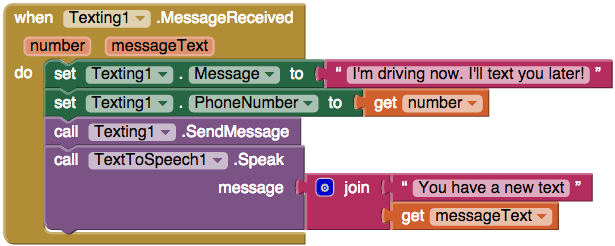
\includegraphics[width=0.95\linewidth]{fig1.png}
	\caption{Blocks for an App Inventor 2 project that automatically respond to texts received with a predefined message and reads the received text aloud.}
	\label{example_blocks}
\end{figure}

There have been two main versions of App Inventor. App Inventor Classic (also known as App Inventor 1) was released in 2009 and ran its blocks editor in a separate Java application. In late 2013, App Inventor 2 (AI2) was released; the Javascript blocks editor now runs in a web browser. As of February 2015, 90\% of the 100,000 active weekly App Inventor users use App Inventor 2. For this reason, this research focuses on App Inventor 2 data \cite{naming:turbak}.

App Inventor is taught to a broad audience, ranging from grade school to college. Reports on courses taught depict App Inventor being used to create very diverse apps. These apps range from apps that discourage texting while driving, to apps that track school buses \cite{thinking:turbak}, to apps that organize community service cleanups \cite{democratizing:wolber}. The pattern we observe is that App Inventor enables "situated computing" \cite{situated:gershman}. This quarter-century old concept suggests that the convergence of computing, connectivity, and content enables users to harness computing to bridge the gap between intentions and actions. App Inventor lets people leverage their mobile devices to solve everyday problems they encounter.

App Inventor also has copious resources for self-learners, typically in the form of self-contained tutorials. A survey of 129,130 self-selected App Inventor users found that 73\% of respondents used App Inventor at home, suggesting a significant portion of App Inventor users learn to use the service on their own and not in a formal learning environment. The App Inventor resources page includes 26 tutorials ranging from beginner to advanced difficulty \cite{ai_tutorials}. These tutorials typically involve creating an entire functioning app from start to finish. Each tutorial typically focuses on either introducing a new component or additional functionality for a previously introduced component.

To date, over 3.1 million users from 195 countries have created over 8.3 million apps with the MIT App Inventor service \cite{ai_home}.


\subsection{Objective}
The goal of this paper is to evaluate the learnability and capability of App Inventor to create apps of differing functionality by analyzing the apps created with App Inventor. We define the learnability as the ease of learning to use the App Inventor service to create an app. When referring to capability, we refer to the extent of App Inventor potential that is realized by users to implement certain functionality.

A guiding principle to the creation of a programming environment is the idea of a “low floor, high ceiling” \cite{CT:Grover}. That is, the environment must be learnable enough such that beginners can easily create a functioning program (low floor), but also have extensible capabilities such that advanced users can also benefit (high ceiling). We are particularly interested in comparing the learnability and capability of App Inventor for creating apps of differing functionality.

We analyze a random sample of projects and group them based on the types of components used in the app. We then look at both the number of unique blocks in projects. We use this grouping and this metric to evaluate how well suited the App Inventor environment is to creating apps with various functionalities.

In this paper, we explain our technical approach of extracting information from raw project data, filtering and grouping projects, and comparing the \emph{sophistication} of the projects we grouped given our metric (number of unique blocks).  We then discuss our findings in the context of the App Inventor service and its teaching resources.


\subsection{Previous Work}
Prior to this work, analysis of App Inventor Classic data has been done by \cite{blocks:okerlund}. Some of the notable findings:
\begin{itemize}
	\item 30\% of projects have no blocks and therefore are not functional.
	\item Nearly 50\% of users do not have a single block or component in their projects.
	\item 51\% of procedures are only called 0 or 1 time.
\end{itemize}
This data indicates that a large number of App Inventor Classic projects were never completed. It was suggested that a major contributing factor is the usability of the service. Whereas App Inventor 2 is a single-page web service, App Inventor Classic required the deployment of an external Java service to program the app. The high proportion of projects without blocks motivated the usability changes of the blocks in App Inventor 2.

A field study of end-user programming on mobile devices was conducted for TouchDevelop, a programming environment that enables users to develop mobile applications directly from mobile devices \cite{TouchDevelop:Li}. The study's objectives included measuring users' progress in developing TouchDevelop scripts. Researchers found that 71.3\% of users learned a few features about the environment initially and then stopped learning new features. To encourage more continuous learning, researchers suggested providing an adaptive tutoring system that recommends tutorials similar to the kind of script a user is developing and avoids tutorials that cover features users already know. As discussed later in the paper, our findings suggest that App Inventor may also have a similar situation where users tend to only learn a subset of features available to them.


\section{Technical Approach}

We extracted features from a random sampling of App Inventor 2 projects. We grouped projects based on their functionality by considering the components they contain. We then measured the \emph{total number of unique blocks} (NOUB) in the projects to determine the sophistication they exhibit. Finally, we examined the distribution of the NOUB in each group to answer our research question.


\subsection{Data Source}
Our source data is 5,228 App Inventor 2 projects selected at random from the total corpus of 8.3 million projects. We randomly selected projects according to their unique project IDs. The 5,228 projects selected come from 5,174 users, suggesting that randomization was accomplished. Given the size of the dataset and the randomness of the selection, we assume that the sample is representative of App Inventor 2 projects as a whole. We used Pandas, a Python data analysis library, for our data processing \cite{pandas}.


Of the 5,228 projects sampled...
\begin{itemize}
	\item At least 16.4\% (859 projects) are recreations of App Inventor tutorials. These recreations of the step-by-step tutorials were identified by matching project names. We considered only the 26 tutorials from the MIT App Inventor website, although many other tutorials made by other groups and individuals exist \cite{course_in_box} \cite{imagnity}. Projects that are recreations of these tutorials are filtered out of our dataset.
	\item 21\% (1,107 projects) are \emph{Certainly Static}; that is, they are guaranteed to be apps that have no behavior and never change state. If a project has no components, then there is nothing the user can interact with or for the app to do, so the project must be static. For an app to be interactive and have behavior, in addition to at least one component, it must also have at least two blocks: One to handle an event and one to respond to that event. Figure 2 shows an example of a simple action from two blocks. No functionality can occur with fewer than two blocks. We say an app is Certainly Static if it either has no components or has fewer than two blocks.
\end{itemize}

\begin{figure}[h!]
	\centering
	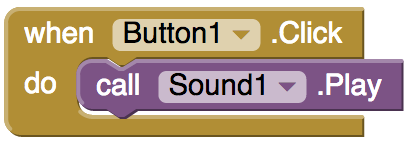
\includegraphics[width=0.55\linewidth]{simple_blocks.png}
	\caption{The simplest app behavior requires at least two blocks: An event handler and a resulting action. Here, a sound is played when a button is pressed.}
	\label{basic_blocks}
\end{figure}

We chose to filter out the Certainly Static projects as well as projects that are recreations of tutorials, so our analysis was run over the remaining 3,289 projects. While we can guarantee that the removed projects are static, we cannot guarantee the remaining projects have behavior, as their blocks may not be connected in a manner that allows for any behavior. For the purpose of analysis, we assume the remaining 3,289 projects have behavior and are not recreations of tutorials.

\subsection{Feature Extraction}
We focused primarily on quantitative features for our analysis, particularly the number of each type of component in a project, and the number of each type of block. This information exists in the source code of the projects. 


Features Extracted from Projects:
\begin{itemize}
	\item Project Name
	\item User Name (anonymized)
	\item Number of Components by Type
	\item Number of Blocks by Type
\end{itemize}

\subsection{Grouping Projects}
We use the components within a project to group projects by functionality. The palette in App Inventor organizes components by functionality, or behavior, and places each group in its own "drawer" (Figure 3). Because the palette neatly organizes components into categories , we use it to define our groups. If an app has components from multiple palette drawers, it may be categorized in multiple groups, as explained later in this section.


\begin{figure}[h!]
	\centering
	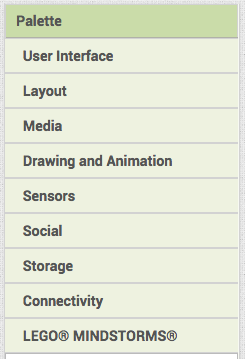
\includegraphics[width=0.4\linewidth]{palette.png}
	\caption{The palette groups components into categories. We use these categories to group projects by functionality.}
	\label{palette}
\end{figure}

We follow the palette drawers to define our groups, with two notable changes: Disregarding the entire "Layout" component drawer and the sound and clock components. 

Layout components were removed because they do not add additional functionality and are therefore irrelevant for our groupings. These components only enable users to change the arrangement of an app's visual components. Since we group projects by their functionality and layout components add no additional behavior to apps, they are disregarded.

The sound and clock components were removed to improve the differentiation between functionality groups. The sound component plays a sound whenever the user specifies. Examples include playing a "meow" when an image of a cat is pressed and playing a famous speech in a historical quiz app. The clock component enables apps to keep track of time. Uses for this vary from keeping time in a stopwatch app to periodically moving a sprite in a game app. Because the sound and clock components have such broad uses, they do not help differentiate apps' behaviors between groups and are also excluded in the consideration of functionality groups.

We categorize the 3,289 apps into eight groups. \emph{Basic} apps only contain User Interface components. Apps in the \emph{Media, Drawing, Sensor, Social, Storage, Connectivity}, and \emph{Lego} groups contain at least one component from that respective drawer in the palette. This categorization allows for overlap, as projects that contain components from multiple palette drawers are placed in multiple groups. For example, a project that uses both Bluetooth (connectivity) and Twitter (social) components would be labeled both Connectivity and Social. The exception is the Lego group, which we deem to be a disjoint group because of the specificity of the components. Lego components are solely for integration with Lego Mindstorms \cite{lego}; if a project contains a Lego component, it is only grouped as Lego, regardless of other components it may contain. 

Reiterating, Basic and Lego groups are disjoint from other groups and each other. Other groups may overlap. Table 1 provides a description of each group, the condition for a project to be in that group, and example apps and components from each group.

\begin{table}[h!]
% increase table row spacing, adjust to taste
\renewcommand{\arraystretch}{1.3}
% if using array.sty, it might be a good idea to tweak the value of
% \extrarowheight as needed to properly center the text within the cells
\caption{Functionality Groupings}
\label{table_groups}
\centering
% Some packages, such as MDW tools, offer better commands for making tables
% than the plain LaTeX2e tabular which is used here.
%\begin{tabular}{ c | c | | c | c}
\begin{tabular}{| p{0.13\linewidth} | p{0.28\linewidth} | p{0.20\linewidth} | p{0.2\linewidth} | }
\hline

Group Name &  Description of App Functionality \{Example App\} & Condition & Example Components\\
\hline
\hline
Basic & Only basic user interface components \{Splits bill amongst certain number of people\} 
 &Only User Interface Components & Button, Image, Label, Notifier, Textbox \\
\hline

Media & Playing/recording audio or video \{Click on picture of politician to hear their famous speech\} & At least 1 media component (excluding "sound") &Camera, TextToSpeech, VideoPlayer, MusicPlayer \\
\hline

Drawing
&Use screen as canvas for drawing \{Draw on picture of cat\}
&At least 1 drawing component
&Canvas, Ball, ImageSprite\\
\hline

Sensor
&Response to phones’ sensors \{Shake phone to roll a die\}
&At least 1 sensor component (excluding "clock')
&Accelerometer Sensor, Location Sensor, NearField (NFC)\\
\hline


Social
&Communication via phone or web \{Click on a person’s picture to call or text them\}
&At least 1 social component
&Texting, Twitter, PhoneCall\\
\hline

Storage
&Saving information \{Add items to grocery list and save list\}
&At least 1 storage component
&TinyDB, Fusiontables Control, File\\
\hline

Connectivity
&Networking with other apps and phones \{Get latest stock quotes from web\}
&At least 1 connectivity component
&ActivityStarter, BluetoothClient, Web\\

\hline
Lego
&Control Lego Mindstorm kits \{Remote control for Lego Mindstorm NXT robot\}
&At least 1 lego components
&NxtDrive, NxtLightSensor\\
\hline

\end{tabular}
\end{table}

We use the components to group projects and the blocks to measure the sophistication of them.

\subsection{Measuring Programmatic Sophistication}
We define the \emph{sophistication} of an App Inventor project as a measurement of the skill involved to create an app as evidenced by the blocks used. More sophisticated projects tend to reflect good coding practices, such as code reuse through procedures. A more sophisticated app tends to either use more components or use blocks corresponding to these components more effectively. 

Code reuse is a particular focus in our measure of sophistication. For example, consider the case where two functionally similar projects exist and Project A copies the same code in three locations whereas Project B defines a procedure and calls that procedure three times. We argue Project B is more sophisticated as it leverages code reuse in the form of procedures. Project A has a greater number of blocks, but Project B has a greater number of \emph{unique} blocks (NOUB) with the block to define a procedure and the block to call a procedure included. A project that appropriately uses a procedure rather than copying blocks shows evidence of greater computational thinking and therefore greater sophistication \cite{rubric:sherman}, even if the resulting apps have identical functionality.

We measure programmatic sophistication of App Inventor projects by looking at the NOUB that exist in the project. We choose the NOUB instead of the total number of blocks so the measure of sophistication is not affected by redundant code. 

\section{Results}
We show the division of the projects into groups then show the distribution of the number of unique blocks (NOUB) in projects of each group. 


\subsection{Grouping}
After grouping projects by functionality, we find that 78.1\% of projects can be categorized into exactly one group. The remaining projects were categorized across multiple groups (see 2C for explanation). The 3,289 projects were categorized into 4,282 groups; on average, a project fit into 1.3 groups. Figure 4 shows the division of projects into groups.

Based on the distribution of projects into groups, we observe a relationship between this distribution and App Inventor tutorials. Due to the simplicity of functionality that defines the group, the largest group is the Basic group. Over half of the App Inventor beginner tutorials involve the creation of a drawing app \cite{ai_tutorials} and we see that the Drawing group is the second largest group. These observations suggest that the large number of drawing apps users create are projects that are very similar in functionality to tutorials. The Lego group is the smallest, containing only 0.7\% (27 projects) of the data. One likely explanation is the additional hardware requirement (Lego Mindstorm kits) to use an app grouped as Lego. Another is that there are no official tutorials for Lego projects, so users do not have a way to learn how to use the Lego components. We hypothesize that the number of projects in each functionality group correlates with the number of functionally similar tutorials available. We further address this in our Discussion section.


\begin{figure}[h!]
	\centering
	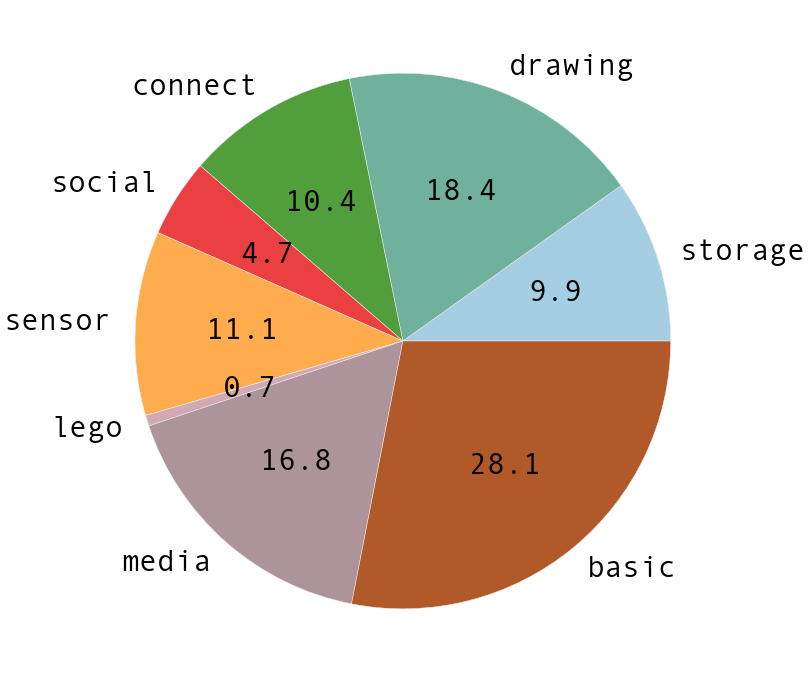
\includegraphics[width=0.9\linewidth]{pie_group.png}
	\caption{Size of Functionality Groups. 78.1\% of projects are categorized into exactly one group, with the others categorized across multiple groups.}
	\label{DistributionOfGroups}
\end{figure}

\subsection{Number of Unique Blocks}
We plot the distribution of the NOUB in each group and compare these subsets of projects to each other and to the entire set of projects. Figure 5 and Table 3 show the NOUB for projects within each group, as well as the distribution for all projects ("All" in Figure 5). 

Each subset and the entire set of projects exhibits a positive skew, suggesting that each group contains a few outlier projects that have a significantly greater NOUB and are likely well-developed apps.

The Storage group has the greatest median NOUB, the widest distribution, and contains the project with the most unique blocks, suggesting that apps that utilize storage functionality tend to be the most advanced and sophisticated. This could be because storage components often require structures such as lists and loops to leverage its more advanced functionality. An example would be using a loop to iterate over the keys and values in a database (TinyDB) component and saving values into a list.  

The wide lower quartile and narrow overall distribution of the Lego group suggests its capabilities are limited. The Lego group has a wide lower quartile (lower whisker in Figure 5) relative to its narrow distribution, suggesting that even a simple project involving Lego components requires more unique blocks to create. The narrow distribution and low median for the Lego group suggests that the capability to create Lego apps is limited. The need for more unique blocks to create even a simple app with Lego components and the limited functionality of these apps suggests that developing these apps is not as intuitive and therefore more difficult to create.

Because 21.9\% of projects fit into multiple groups, one project can be represented in multiple plots. This is most evident in the outliers. The greatest outlier is a password keeper app with 56 unique blocks in it; it is categorized as a Storage, Connectivity, and Media app because it has components of each of those types.



\begin{figure}[h!]
	\centering
	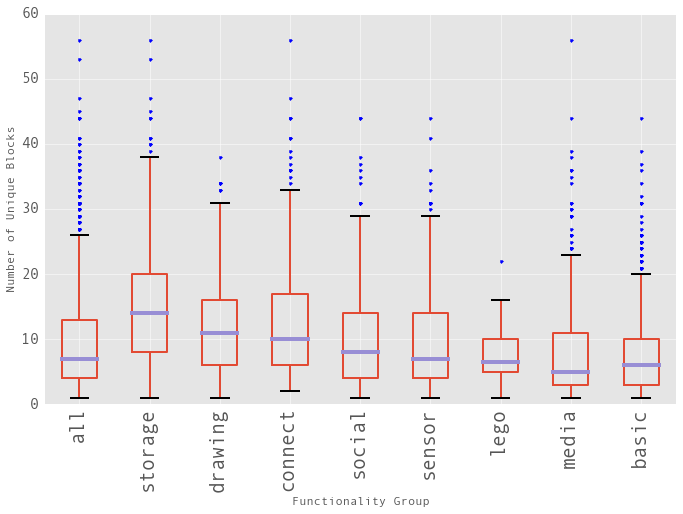
\includegraphics[width=1\linewidth]{boxplot.png}
	\caption{Distribution of Number of Unique Blocks by Functionality Group}
	\label{Distribution of Num of Unique Blocks}
\end{figure}

\begin{table}[h!]
% increase table row spacing, adjust to taste
\renewcommand{\arraystretch}{1.3}
% if using array.sty, it might be a good idea to tweak the value of
% \extrarowheight as needed to properly center the text within the cells
\caption{Summary Statistics for the Number of Unique Blocks by Group}
\label{table_noub_stats}
\centering
% Some packages, such as MDW tools, offer better commands for making tables
% than the plain LaTeX2e tabular which is used here.
%\begin{tabular}{ c | c | | c | c}
\begin{tabular}{| p{0.043\linewidth} | p{0.043\linewidth} | p{0.06\linewidth} | p{0.07\linewidth} | p{0.067\linewidth} | p{0.05\linewidth} | p{0.048\linewidth} | p{0.036\linewidth} | p{0.05\linewidth} | p{0.04\linewidth}|}
%\begin{tabular}{| [ | c | c | c | c | c | c | c | c | c |}
\hline

&all
&storage
&drawing
&connect.
&social
&sensor
&lego
&media
&basic\\
\hline \hline

med.
&7
&14
&11
&10
&8
&7
&6.5
&5
&6\\
\hline

mean&
9.17&
15.40&
11.29&
12.34&
10.19&
9.80&
7.86&
8.14&
9.17\\
\hline

std. dev.&
7.11&
9.61&
6.83&
8.79&
8.73&
7.43&
4.86&
6.94&
5.80\\
\hline

max (w/o outliers)&
26.5&
38.0&
31.0&
33.5&
29.0&
29.0&
17.5&
23.0&
20.5\\
\hline

\# outliers&
90&
11&
6&
14&
10&
12&
1&
26&
41\\
\hline


\hline

\end{tabular}
\end{table}

\section{Discussion}
We critique our use of the number of unique blocks as a metric for measuring sophistication and analyze the intuitiveness of creating different types of apps with App Inventor. We then discuss the capability realized by end-users. Finally, we relate this discussion on learnability and capability to App Inventor tutorials.

\subsection{Analysis of Metric}
When measuring the sophistication of projects, our challenge is to ensure that project categories do not bias our metrics. That is, our measurement of app sophistication is not affected simply because apps include a specific component and hence fall under a certain group. We want to measure apps solely according to the sophistication exhibited by the blocks. We argue that our metric of the NOUB is not dependent on the functionality of the app and is therefore a generalizable metric of programmatic sophistication.

Because App Inventor has component-specific blocks, the NOUB in a project is not directly dependent on its components. App Inventor is event-driven, meaning the programming of App Inventor involves responding to an action, or event, from a component. Each component has its own unique blocks to handle events, get and set attributes of the component, and call component functions. Because of this, using one component instead of another does not inherently change the NOUB in a project. App Inventor blocks respond to events, get/set attributes, and trigger component actions. Figure 6 shows an example of custom component blocks handling an event, calling a function, and setting an attribute. Because of App Inventor's component-specific blocks, the NOUB in a project is a suitable metric to measure the sophistication of projects.

\begin{figure}[h!]
	\centering
	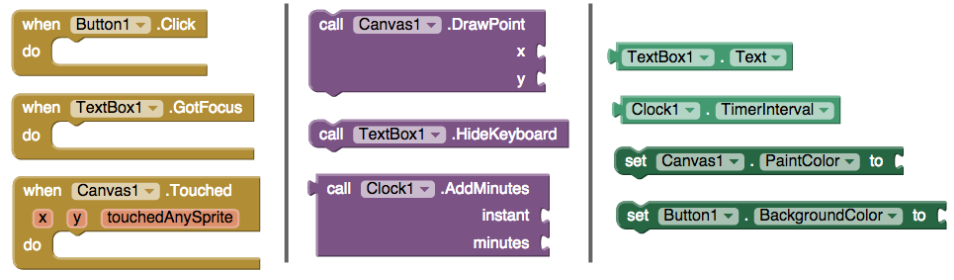
\includegraphics[width=0.8\linewidth]{component_blocks.png}
	\caption{Component-Specific Blocks. The button component has a block to handle being pressed, the sound component has a block to play a sound, and the canvas component has block to set the color.}
	\label{component_specific_blocks}
\end{figure}

Because the NOUB does not systematically vary according to the components used in the projects, we find this metric suitable for our analysis.

\subsection{Learnability}
We claim a group to have high learnability if it does not require many different blocks to create a project. If a group has high learnability, we expect many projects to be categorized into that group. We define a \emph{learnability score} of a group as the number of projects in the group divided by the the median number of unique blocks for that group. The results for the different groups are depicted in Figure 7. 

\begin{figure}[h!]
	\centering
	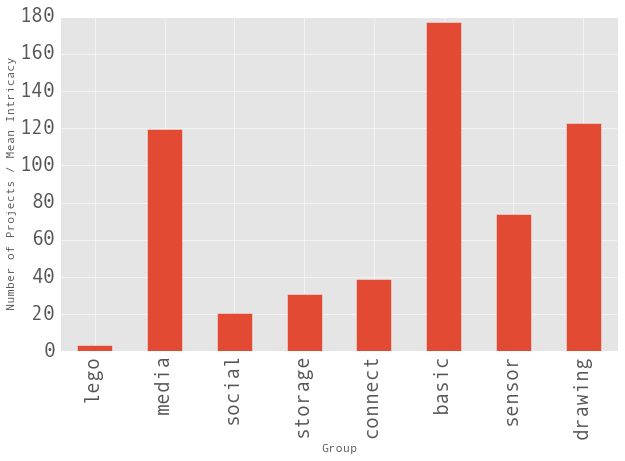
\includegraphics[width=1\linewidth]{learnability.png}
	\caption{Learnability Score (Ratio of the Number of Projects to Median Number of Unique Blocks) of Functionality Groups}
	\label{LearnabilityScore}
\end{figure}

Apps in the Basic group have the highest learnability score and are therefore the easiest to learn. This is not surprising because we narrowly define the Basic group to contain apps that only use user interface components. The Drawing and Media groups also have high learnability scores. This is likely because the tutorials heavily focus on creating Drawing apps and Media apps. We argue that the learnability score is influenced by the beginner tutorials and address this later in the Discussion section.

\subsection{Capability}
We focus our discussion on \emph{realized} capability, or the maximum potential of App Inventor that users actually reach. We are not referring to the "true" capability of App Inventor, the capability that is technically possible but in practice almost never implemented by users. 

To assess the realized capabilities for App inventor to create apps of certain functionalities, we are interested in the projects in each group that have the greatest sophistication (greatest NOUB). It is these projects that best reflect the capability of App Inventor to accomplish certain functionality. We choose to look at the the maximum NOUB in each group excluding outlier projects. This is the end of the upper whiskers in Figure 5 and also shown in Table 2. We argue that these apps best represent the capability realized by App Inventor users.

We say that a greater NOUB correlates with the ability to use App Inventor to create apps that have more advanced functionality. Having the least capability are Lego apps, with the narrowest distribution and lowest maximum NOUB. On the highest end of the spectrum are Storage apps which leverage databases or tables to persist data.

We see that apps with the greatest capability tend to connect to other mobile features or apps or with the web. Storage and connectivity apps have the highest maximum NOUB so we say these functionalities have the greatest realized capability to be extensible. Storage apps connect to some form of data persistence (database, table, file). Connectivity apps connect with other apps in the phone, utilize Bluetooth, and connect with the web. While Social apps connect to other features in the phone (contact list, texting, etc.) or with web services such as Twitter, their realized capabilities are lower. This could be a result of a lack of learning resources relating to this particular functionality limiting the known capability of the group. In general, we see that App Inventor’s most advanced apps tend to connect to the web and other apps and services. This opportunity for extensibility while maintaining the scaffolding that is the App Inventor environment is critical to an environment that fosters computational thinking \cite{checklist:repenning}.

\subsection{Relation to Learning Resources}
The close correlation between learning scores and the sequence of tutorials suggests that users build apps based on knowledge from the tutorials that they complete. On the App Inventor website, tutorials are displayed as a list in sequential order, starting with \emph{Beginner} tutorials and ending with \emph{Advanced} tutorials. Table 4 shows the number of projects that were found to be tutorial recreations as well as the number of tutorials for each group.

Most users tend to start with the beginner tutorials, but the number of tutorials followed until users create their own original projects varies. The earlier a tutorial appears in the sequence on the website, the more users will use it as evidenced by the high proportion of tutorial recreations that are of beginner difficulty (Table 3). We see Drawing, Media and Sensor apps appear as beginner tutorials; these groups also account for most of the tutorial recreations and have the highest learnability scores. There are no Lego tutorials, and the very low learnability score reflects that. Although there are six tutorials involving Storage functionality, they are classified as Intermediate and Advanced, so there are fewer recreations of these tutorials. The Connectivity and Social groups also have a low learnability score and few projects recreate these tutorials. We see that lower learnability scores correlate to groups that have fewer tutorial recreations; we see that the farther along a tutorial exists in the sequence, the fewer times it will be recreated.

\begin{table}[h!]
% increase table row spacing, adjust to taste
\renewcommand{\arraystretch}{1.3}
% if using array.sty, it might be a good idea to tweak the value of
% \extrarowheight as needed to properly center the text within the cells
\caption{Number of Apps that are Tutorial Recreations \{Number of Tutorials\} by Functionality Group and Difficulty Level}
\label{table_tutorial_group}
\centering
% Some packages, such as MDW tools, offer better commands for making tables
% than the plain LaTeX2e tabular which is used here.
%\begin{tabular}{ c | c | | c | c}
%\begin{tabular}{| p{0.15\linewidth} | p{0.15\linewidth} | p{0.15\linewidth} | p{0.15\linewidth} |  p{0.15\linewidth} | p{0.15\linewidth} | }
%\begin{tabular}{|c|c|c|c|c|c|}
\begin{tabular}{| l | l | l | l | l | l |}
\hline
\multicolumn{2}{|c|}{}&
\multicolumn{3}{|c|}{Tutorial Difficulty}&
\\
\hline
\multicolumn{2}{|c|}{}&
Beginner&
Intermediate&
Advanced&
Total\\
\hline
\multirow{9}{*}{Groups} 
&All& 683 \{9\} & 95 \{10 \} & 54 \{7\} & 832 \{26\}\\

&Storage& 0 \{0\}& 5 \{1\} & 48 \{5\} & 53 \{6\}\\

&Connectivity & 0 \{0\} & 9 \{1\} & 26 \{2\} & 35 \{3\}\\

&Drawing &447 \{4\} &70 \{5\} & 5 \{2\} &522 \{11\} \\

&Social & 0 \{0\} &6 \{1\} & 0 \{0\} &6 \{1\}\\

&Sensor &142 \{2\} & 0 \{0\} & 35 \{4\} &177 \{6\}\\

&Lego &0 \{0\} &0 \{0\} &0 \{0\} &0 \{0\}\\

&Media &198 \{2\} &4 \{3\} &0 \{0\} &202 \{5\}\\

&Basic &81 \{1\} &11 \{1\} &0 \{0\} &92 \{2\}\\
\hline


\end{tabular}
\end{table}

This correlation between the number of tutorial recreations and the learnability scores for a given functionality suggests that users build off the knowledge from tutorials when creating an app. The relationship between few tutorial recreations for groups and low learnability scores suggests that if users do not learn a concept directly from a tutorial, they tend to have trouble generalizing knowledge from other tutorials. Therefore, users tend not to create apps that are functionally different from completed tutorials. This is troublesome as \cite{TouchDevelop:Li} noted that 71.3\% of users of the similar TouchDevelop programming environment tended to learn only a few features initially and not seek to learn more later. We see that users do not complete enough tutorials to gain a thorough understanding to create apps of differing functionality with App Inventor, so there exists a need to make tutorials more available and the knowledge from them more generalizable.

To better prepare users to create apps with more diverse functionality, we propose changes to the App Inventor learning resources to ensure tutorials are more accessible and contain more transferrable knowledge. We consider the following changes to App Inventor tutorials:
\begin{itemize}
	\item Avoid Pre-defined Paths for Tutorials: As of now, App Inventor tutorials exist as a list where tutorials often do not build off of knowledge from previous ones. So, we suggest that tutorials be offered in such a way that users do not feel obligated to follow an unnecessary predefined "path" when recreating tutorials. Instead, users should be more inclined to select tutorials relevant to their interests.
	\item Organizing Learning Resources: Because learning resources tend to be separate from each other on the MIT App Inventor website, users may not know where to go when they encounter a problem, or they may not even know given resources exist. In example, concept cards, which explain specific concepts, can serve as quick references for users \cite{concept_cards}. They are placed with the teaching resources on the App Inventor website, entirely separate from tutorials. Ensuring that users have a centralized and organized point to access resources would better support users.
	\item Adaptive Tutorials: Suggested in a similar context by \cite{TouchDevelop:Li}, an adaptive tutoring system that recommends resources relevant to what the user is creating and avoids resources of concepts already learned or implemented.

\end{itemize}


%%%%%%%%%%


\section{Conclusion}
In this paper, we evaluate the learnability (low floor) and capability (high ceiling) of App Inventor, a web-based environment that enables users to create mobile apps. From our sample of 5,228 apps, we filtered out Certainly Static apps and apps that are recreations of our tutorials and grouped apps by similar functionality. We then measured the number of unique blocks for projects in each group and compared the groups. Our findings include (1) there exists a strong correlation between the learnability and the number of tutorial recreations for a given functionality; (2) users tend to follow tutorials sequentially and therefore often do not complete more than beginner tutorials; (3) users tend to develop apps that are functionally similar to completed tutorials. Based on these findings, we suggest that the realized capabilities of App Inventor are limited by the provided learning resources. We have provided a list of recommendations for improving these learning resources for end-users.

The existence of non-functional projects and recreations of tutorials in our dataset offer opportunities for future work. While we filtered out projects that were certainly static by ensuring all projects had the minimum number of components and blocks, there still exist projects that do not have any functionality. Disregarding blocks that are not connected to other blocks and components with no programmed functionality would better filter out the non-functional projects. And although we filter out projects that are recreations of tutorials by matching project names, a more robust method of identifying projects that are merely recreations would improve the dataset. We could focus analysis on specific advanced structures more closely tied with computational thinking such as iterators and procedures, as defined by \cite{paper:sherman}. Finally, we plan on analyzing user and temporal data, investigating how users and their apps develop over time.


\section*{Acknowledgments}
We thank Jeffery Schiller (MIT App Inventor) for helping collect the data, Ilaria Liccardi (MIT) and Franklyn Turbak (Wellesley College) for helping guide the analysis, and Aubrey Colter (MIT App Inventor) for significantly helping proofread this paper. 

This research is funded by the MIT EECS - Google Research and Innovation Scholarship as part of the 2014-15 MIT SuperUROP Program. 




% trigger a \newpage just before the given reference
% number - used to balance the columns on the last page
% adjust value as needed - may need to be readjusted if
% the document is modified later
%\IEEEtriggeratref{8}
% The "triggered" command can be changed if desired:
%\IEEEtriggercmd{\enlargethispage{-5in}}

% references section

% can use a bibliography generated by BibTeX as a .bbl file
% BibTeX documentation can be easily obtained at:
% http://www.ctan.org/tex-archive/biblio/bibtex/contrib/doc/
% The IEEEtran BibTeX style support page is at:
% http://www.michaelshell.org/tex/ieeetran/bibtex/
%\bibliographystyle{IEEEtran}
% argument is your BibTeX string definitions and bibliography database(s)
%\bibliography{IEEEabrv,../bib/paper}
%
% <OR> manually copy in the resultant .bbl file
% set second argument of \begin to the number of references
% (used to reserve space for the reference number labels box)
%\bibitem{IEEEhowto:kopka}
%H.~Kopka and P.~W. Daly, \emph{A Guide to \LaTeX}, 3rd~ed.\hskip 1em plus
%  0.5em minus 0.4em\relax Harlow, England: Addison-Wesley, 1999.

%\newpage

%\bibitem{IEEEhowto:kopka}
%H.~Kopka and P.~W. Daly, \emph{A Guide to \LaTeX}, 3rd~ed.\hskip 1em plus
%  0.5em minus 0.4em\relax Harlow, England: Addison-Wesley, 1999.  

\bibliographystyle{IEEEtran}
\bibliography{bibfile}

% An example of a floating figure using the graphicx package.
% Note that \label must occur AFTER (or within) \caption.
% For figures, \caption should occur after the \includegraphics.
% Note that IEEEtran v1.7 and later has special internal code that
% is designed to preserve the operation of \label within \caption
% even when the captionsoff option is in effect. However, because
% of issues like this, it may be the safest practice to put all your
% \label just after \caption rather than within \caption{}.
%
% Reminder: the "draftcls" or "draftclsnofoot", not "draft", class
% option should be used if it is desired that the figures are to be
% displayed while in draft mode.
%
%\begin{figure}[!t]
%\centering
%\includegraphics[width=2.5in]{myfigure}
% where an .eps filename suffix will be assumed under latex, 
% and a .pdf suffix will be assumed for pdflatex; or what has been declared
% via \DeclareGraphicsExtensions.
%\caption{Simulation Results}
%\label{fig_sim}
%\end{figure}

% Note that IEEE typically puts floats only at the top, even when this
% results in a large percentage of a column being occupied by floats.


% An example of a double column floating figure using two subfigures.
% (The subfig.sty package must be loaded for this to work.)
% The subfigure \label commands are set within each subfloat command, the
% \label for the overall figure must come after \caption.
% \hfil must be used as a separator to get equal spacing.
% The subfigure.sty package works much the same way, except \subfigure is
% used instead of \subfloat.
%
%\begin{figure*}[!t]
%\centerline{\subfloat[Case I]\includegraphics[width=2.5in]{subfigcase1}%
%\label{fig_first_case}}
%\hfil
%\subfloat[Case II]{\includegraphics[width=2.5in]{subfigcase2}%
%\label{fig_second_case}}}
%\caption{Simulation results}
%\label{fig_sim}
%\end{figure*}
%
% Note that often IEEE papers with subfigures do not employ subfigure
% captions (using the optional argument to \subfloat), but instead will
% reference/describe all of them (a), (b), etc., within the main caption.


% An example of a floating table. Note that, for IEEE style tables, the 
% \caption command should come BEFORE the table. Table text will default to
% \footnotesize as IEEE normally uses this smaller font for tables.
% The \label must come after \caption as always.

%\begin{table}[!t]
%% increase table row spacing, adjust to taste
%\renewcommand{\arraystretch}{1.3}
%% if using array.sty, it might be a good idea to tweak the value of
%% \extrarowheight as needed to properly center the text within the cells
%\caption{An Example of a Table}
%\label{table_example}
%\centering
%% Some packages, such as MDW tools, offer better commands for making tables
%% than the plain LaTeX2e tabular which is used here.
%\begin{tabular}{|c||c|}
%\hline
%One & Two\\
%\hline
%Three & Four\\
%\hline
%\end{tabular}
%\end{table}


% Note that IEEE does not put floats in the very first column - or typically
% anywhere on the first page for that matter. Also, in-text middle ("here")
% positioning is not used. Most IEEE journals/conferences use top floats
% exclusively. Note that, LaTeX2e, unlike IEEE journals/conferences, places
% footnotes above bottom floats. This can be corrected via the \fnbelowfloat
% command of the stfloats package.




% conference papers do not normally have an appendix


% use section* for acknowledgement



% trigger a \newpage just before the given reference
% number - used to balance the columns on the last page
% adjust value as needed - may need to be readjusted if
% the document is modified later
%\IEEEtriggeratref{8}
% The "triggered" command can be changed if desired:
%\IEEEtriggercmd{\enlargethispage{-5in}}

% references section

% can use a bibliography generated by BibTeX as a .bbl file
% BibTeX documentation can be easily obtained at:
% http://www.ctan.org/tex-archive/biblio/bibtex/contrib/doc/
% The IEEEtran BibTeX style support page is at:
% http://www.michaelshell.org/tex/ieeetran/bibtex/
%\bibliographystyle{IEEEtran}
% argument is your BibTeX string definitions and bibliography database(s)
%\bibliography{IEEEabrv,../bib/paper}
%
% <OR> manually copy in the resultant .bbl file
% set second argument of \begin to the number of references
% (used to reserve space for the reference number labels box)
%\bibitem{IEEEhowto:kopka}
%H.~Kopka and P.~W. Daly, \emph{A Guide to \LaTeX}, 3rd~ed.\hskip 1em plus
%  0.5em minus 0.4em\relax Harlow, England: Addison-Wesley, 1999.



% that's all folks
\end{document}
